\documentclass{if-beamer}

% --------------------------------------------------- %
%                  Presentation info	              %
% --------------------------------------------------- %
\title[Lecture 22]{Integration}
\subtitle{Richardson Extrapolation and Romberg Integration}
\author{Ashley Gannon}
\date{Fall 2020}
\logo{

\includegraphics[scale=0.08]{figures/FSULogo.png}
}
\subject{Presentation subject}

% --------------------------------------------------- %
%                    Title + Schedule                 %
% --------------------------------------------------- %
\begin{document}

\begin{frame}
  \titlepage
\end{frame}
% --------------------------------------------------- %
%                      Presentation                   %
% --------------------------------------------------- %
\section{Richardson Extrapolation}

\begin{frame}[t]
\frametitle{Richardson Extrapolation}
\textit{Richardson extrapolation} methods improve the results of numerical integration by using two estimates of an integral to compute a third, more accurate approximation. \\\vspace{10pt}
\end{frame}

\begin{frame}[t]
	\frametitle{Richardson Extrapolation}
	\textit{Richardson extrapolation} methods improve the results of numerical integration by using two estimates of an integral to compute a third, more accurate approximation. \\\vspace{10pt}
	We'll do examples involving successive iterates of the Trapezoidal Rule. \\\vspace{10pt}
\end{frame}

\begin{frame}[t]
	\frametitle{Richardson Extrapolation}
	\textit{Richardson extrapolation} methods improve the results of numerical integration by using two estimates of an integral to compute a third, more accurate approximation. \\\vspace{10pt}
	We'll do examples involving successive iterates of the Trapezoidal Rule. \\\vspace{10pt}
	We can represent the error of the Trapezoidal rule by
	$$I = I(h) +E(h)$$
	where $I$ is the exact integral, $I(h)$ is the integral approximation using the Trapezoidal rule, and $E(h)$ is the truncation error
	$$ E \cong -\frac{b-a}{12}h^2\bar{f}^{''}$$ 
	when $h = (b-a)/n$.
\end{frame}


\begin{frame}[t]
	\frametitle{Richardson Extrapolation}
If we make two seperate estimates using segment sizes $h_1$ and $h_2$, we can rewrite
$$I = I(h) +E(h)$$
as 
$$I(h_1) +E(h_1) = I(h_2) +E(h_2)$$	
\end{frame}

\begin{frame}[t]
	\frametitle{Richardson Extrapolation}
	If we make two seperate estimates using segment sizes $h_1$ and $h_2$, we can rewrite
	$$I = I(h) +E(h)$$
	as 
	$$I(h_1) +E(h_1) = I(h_2) +E(h_2)$$
	If we assume that $\bar{f}^{''}$ is constant for any $h$, we have the relation
	$$\frac{E(h_1)}{E(h_2)} \cong \frac{-\frac{b-a}{12}h_1^2\bar{f}^{''}}{-\frac{b-a}{12}h_2^2\bar{f}^{''}} \cong \frac{h_1^2}{h_2^2}$$	
\end{frame}

\begin{frame}[t]
	\frametitle{Richardson Extrapolation}
	If we make two seperate estimates using segment sizes $h_1$ and $h_2$, we can rewrite
	$$I = I(h) +E(h)$$
	as 
	$$I(h_1) +E(h_1) = I(h_2) +E(h_2)$$
	If we assume that $\bar{f}^{''}$ is constant for any $h$, we have the relation
	$$\frac{E(h_1)}{E(h_2)} \cong \frac{-\frac{b-a}{12}h_1^2\bar{f}^{''}}{-\frac{b-a}{12}h_2^2\bar{f}^{''}} \cong \frac{h_1^2}{h_2^2}$$
	Solving for $E(h_1)$,
	$$ E(h_1) = E(h_2)\frac{h_1^2}{h_2^2}$$	
\end{frame}
\begin{frame}[t]
	\frametitle{Richardson Extrapolation}
	If we make two seperate estimates using segment sizes $h_1$ and $h_2$, we can rewrite
	$$I = I(h) +E(h)$$
	as 
	$$I(h_1) +E(h_1) = I(h_2) +E(h_2)$$
	If we assume that $\bar{f}^{''}$ is constant for any $h$, we have the relation
	$$\frac{E(h_1)}{E(h_2)} \cong \frac{-\frac{b-a}{12}h_1^2\bar{f}^{''}}{-\frac{b-a}{12}h_2^2\bar{f}^{''}} \cong \frac{h_1^2}{h_2^2}$$
	Solving for $E(h_1)$,
	$$ E(h_1) = E(h_2)\frac{h_1^2}{h_2^2}$$
	Which we can plug back into the above equation so that the integral approximate is only dependent on $E(h_2)$.
	$$I(h_1) +E(h_2)\frac{h_1^2}{h_2^2} = I(h_2) +E(h_2)$$	
\end{frame}

\begin{frame}[t]
	\frametitle{Richardson Extrapolation}
	If we make two seperate estimates using segment sizes $h_1$ and $h_2$, we can rewrite
	$$I = I(h) +E(h)$$
	as 
	$$I(h_1) +E(h_1) = I(h_2) +E(h_2)$$
	If we assume that $\bar{f}^{''}$ is constant for any $h$, we have the relation
	$$\frac{E(h_1)}{E(h_2)} \cong \frac{-\frac{b-a}{12}h_1^2\bar{f}^{''}}{-\frac{b-a}{12}h_2^2\bar{f}^{''}} \cong \frac{h_1^2}{h_2^2}$$
	Solving for $E(h_1)$,
	$$ E(h_1) = E(h_2)\frac{h_1^2}{h_2^2}$$
	Which we can plug back into the above equation so that the integral approximate is only dependent on $E(h_2)$.
	$$I(h_1) +E(h_2)\frac{h_1^2}{h_2^2} = I(h_2) +E(h_2)$$
	Solving for $E(h_2)$ we have
	$$E(h_2) = \frac{I(h_1)-I(h_2)}{1-\frac{h_1^2}{h_2^2}}$$	
\end{frame}

\begin{frame}[t]
	\frametitle{Richardson Extrapolation}
	Since we are interested in the best approximate for the integral, we will use
	$$ I = I(h_2)+E(h_2)$$
\end{frame}

\begin{frame}[t]
	\frametitle{Richardson Extrapolation}
	Since we are interested in the best approximate for the integral, we will use
	$$ I = I(h_2)+E(h_2)$$
	We can substitute the error we found in the previous slide into this equation to yield 
	$$ I = I(h_2) + \frac{I(h_1)-I(h_2)}{1-\frac{h_1^2}{h_2^2}}$$
\end{frame}

\begin{frame}[t]
	\frametitle{Richardson Extrapolation}
	Since we are interested in the best approximate for the integral, we will use
	$$ I = I(h_2)+E(h_2)$$
	We can substitute the error we found in the previous slide into this equation to yield 
	$$ I = I(h_2) + \frac{I(h_1)-I(h_2)}{1-\frac{h_1^2}{h_2^2}}$$
	The error of this approximate is now $\mathcal{O}(h^4)$, compared to each iteration of the Trapezoidal rule $\mathcal{O}(h^2)$. (Raltson and Rabinowitz, 1978)\\\vspace{10pt} 
\end{frame}

\begin{frame}[t]
	\frametitle{Richardson Extrapolation}
Since we are interested in the best approximate for the integral, we will use
$$ I = I(h_2)+E(h_2)$$
We can substitute the error we found in the previous slide into this equation to yield 
$$ I = I(h_2) + \frac{I(h_1)-I(h_2)}{1-\frac{h_1^2}{h_2^2}}$$
The error of this approximate is now $\mathcal{O}(h^4)$, compared to each iteration of the Trapezoidal rule $\mathcal{O}(h^2)$. (Raltson and Rabinowitz, 1978)\\\vspace{10pt} 
For the special case where the interval is halved, $h_2 = h_1/2 = \frac{b-a}{2n}$, we can simplify our approximate to be
\begin{align*}
I &= I(h_2) + \frac{I(h_1)-I(h_2)}{1-\frac{h_1^2}{(h_1/2)^2}} \quad = I(h_2) + \frac{I(h_1)-I(h_2)}{1-4} = I(h_2) + \frac{I(h_2)}{3} - \frac{I(h_1)}{3} \\
 & = \frac{4}{3}I(h_2)- \frac{1}{3}I(h_1)	
\end{align*}
\end{frame}

\begin{frame}[t]
	\frametitle{Richardson Extrapolation Example}
	Use Richardson Extrapolation to evaluate the integral of\\ $f(x) = 0.2 + 25x-200x^2+675x^3-900x^4+400x^5$ from $a = 0$ to $b = 0.8$. \\\vspace{10pt}
\end{frame}

\begin{frame}[t]
	\frametitle{Richardson Extrapolation Example}
	Use Richardson Extrapolation to evaluate the integral of\\ $f(x) = 0.2 + 25x-200x^2+675x^3-900x^4+400x^5$ from $a = 0$ to $b = 0.8$. \\\vspace{10pt}
	First we will use the trapezoid rule on one segment\\
	$$ h = (0.8-0)/1 = 0.8$$
	$$ f(0.8) = 0.232, \quad f(0) = 0.2$$
	\begin{align*}
		I &\approx h\frac{f(a)+f(b)}{2} = 0.8*\frac{0.232+0.2}{2} \\
		&= 0.1728
	\end{align*}
\end{frame}

\begin{frame}[t]
	\frametitle{Richardson Extrapolation Example}
	Use Richardson Extrapolation to evaluate the integral of\\ $f(x) = 0.2 + 25x-200x^2+675x^3-900x^4+400x^5$ from $a = 0$ to $b = 0.8$. \\\vspace{10pt}
	First we will use the trapezoid rule on one segment\\
	$$ h = (0.8-0)/1 = 0.8$$
	$$ f(0.8) = 0.232, \quad f(0) = 0.2$$
	\begin{align*}
	I &\approx h\frac{f(a)+f(b)}{2} = 0.8*\frac{0.232+0.2}{2} \\
	 &= 0.1728
	\end{align*}
	Next we will halve the interval $h = (0.8-0)/2 = 0.4$, and apply the Trapezoidal rule
	\begin{align*}
	 I &\approx h\frac{f(x_0)+f(x_1)}{2} + h\frac{f(x_1)+f(x_2)}{2}\\
	 &= 0.4\frac{0.2+2.456}{2} + 0.4\frac{2.456+f(0.232)}{2}\\ 
	 &= 1.0688 \\
	\end{align*}
\end{frame}

\begin{frame}
	\frametitle{Richardson Extrapolation Example}
	Use Richardson Extrapolation to evaluate the integral of\\ $f(x) = 0.2 + 25x-200x^2+675x^3-900x^4+400x^5$ from $a = 0$ to $b = 0.8$. \\\vspace{10pt}
	
	Now we can plug these values into our integral approximate
	\begin{align*}
		I &= \frac{4}{3}I(h_2)-\frac{1}{3}I(h_1)\\
		&= \frac{4}{3}1.0688-\frac{1}{3}0.1728\\
		&\approx 1.367467\\
	\end{align*}
	Which is closer to the true value, $1.640533$ than either Trapezoidal rule approximate.
\end{frame}

\begin{frame}[t]
	\frametitle{Richardson Extrapolation Example}
	
	In the same manner, we can use estimates for 2 and 4 segments. \\\vspace{10pt}
	
	For 4 segments
	$$ h = (0.8-0)/4 = 0.2$$
	$$ x_0 = 0, \qquad x_1 = 0.2, \qquad x_2 = 0.4,$$
	$$ x_3 = 0.6, \qquad x_4 =0.8 $$
	Plugging these values into our trapezoid rule, 
	$$ I \approx \frac{h}{2}(f(x_0)+f(x_4)) + h\sum_{i=2}^{4} f(x_i) = 1.4848$$

\end{frame}

\begin{frame}[t]
	\frametitle{Richardson Extrapolation Example}
	
	In the same manner, we can use estimates for 2 and 4 segments. \\\vspace{10pt}
	
	For 4 segments
	$$ h = (0.8-0)/4 = 0.2$$
	$$ x_0 = 0, \qquad x_1 = 0.2, \qquad x_2 = 0.4,$$
	$$ x_3 = 0.6, \qquad x_4 =0.8 $$
	Plugging these values into our trapezoid rule, 
	$$ I \approx \frac{h}{2}(f(x_0)+f(x_4)) + h\sum_{i=2}^{4} f(x_i) = 1.4848$$
	Substituting this and the two segment approximate into 
	\begin{align*}
	I &=\frac{4}{3}1.4848-\frac{1}{3}1.0688\\
	&\approx 1.623467\\
	\end{align*}
	Which is even more accurate than the last approximation.
\end{frame}

\begin{frame}[t]
	\frametitle{Richardson Extrapolation Example}
	These two improved integrals can, in turn, be combined to yield an
	even better value with $\mathcal{O}(h^6)$ . For the special case where the original trapezoidal estimates
	are based on successive halving of the step size, the equation used for $\mathcal{O}(h^6)$ accuracy is
	$$ I = \frac{16}{15}I_m -\frac{1}{15}I_l$$
	where the $I_m$ is the more accurate estimate, $I_l$ is the less accurate estimate. \\\vspace{10pt}
\end{frame}

\begin{frame}[t]
	\frametitle{Richardson Extrapolation Example}
	 These two improved integrals can, in turn, be combined to yield an
	even better value with $\mathcal{O}(h^6)$ . For the special case where the original trapezoidal estimates
	are based on successive halving of the step size, the equation used for $\mathcal{O}(h^6)$ accuracy is
	$$ I = \frac{16}{15}I_m -\frac{1}{15}I_l$$
	where the $I_m$ is the more accurate estimate, $I_l$ is the less accurate estimate. \\\vspace{10pt} For our example, we have
	\begin{align*}
		I & = \frac{16}{15}(1.623467) -\frac{1}{15}(1.367467)\\
		& = 1.640533
	\end{align*}	
Which is the exact integral.
\end{frame}

\section{Romberg Integration}

\begin{frame}[t]
	\frametitle{Romberg Integration}
	Notice the coefficients for
	$$ I = \frac{4}{3}I_m -\frac{1}{3}I_l$$
	and
	$$ I = \frac{16}{15}I_m -\frac{1}{15}I_l$$
	add to 1. \\\vspace{10pt}
	
	You may think of these coefficients as weights. We place a larger weight on the more accurate integral approximation. \\\vspace{10pt}
	
\end{frame}

\begin{frame}[t]
	\frametitle{Romberg Integration}
	Notice the coefficients for
	$$ I = \frac{4}{3}I_m -\frac{1}{3}I_l$$
	and
	$$ I = \frac{16}{15}I_m -\frac{1}{15}I_l$$
	add to 1. \\\vspace{10pt}
	
	You may think of these coefficients as weights. We place a larger weight on the more accurate integral approximation. \\\vspace{10pt}
	
	If we let $k = 1,2,...n$ correspond to the order of accuracy where \\
	\begin{minipage}{0.3\textwidth}
		\begin{table}
			\begin{tabular}{c | c }
				k & L\\
				\hline
				1 & $\mathcal{O}(h^2)$ \\
				2 & $\mathcal{O}(h^4)$ \\
				3 & $\mathcal{O}(h^6)$ \\
				$\vdots$ & $\vdots$ \\
				n & $\mathcal{O}(h^{2n})$ \\
			\end{tabular}
		\end{table}
	\end{minipage}
	\begin{minipage}{0.7\textwidth}
			
	\end{minipage}
\end{frame}

\begin{frame}[t]
	\frametitle{Romberg Integration}
	Notice the coefficients for
	$$ I = \frac{4}{3}I_m -\frac{1}{3}I_l$$
	and
	$$ I = \frac{16}{15}I_m -\frac{1}{15}I_l$$
	add to 1. \\\vspace{10pt}
	
	You may think of these coefficients as weights. We place a larger weight on the more accurate integral approximation. \\\vspace{10pt}
	
	If we let $k = 1,2,...n$ correspond to the order of accuracy where \\
	\begin{minipage}{0.3\textwidth}
		\begin{table}
			\begin{tabular}{c | c }
				k & L\\
				\hline
				1 & $\mathcal{O}(h^2)$ \\
				2 & $\mathcal{O}(h^4)$ \\
				3 & $\mathcal{O}(h^6)$ \\
				$\vdots$ & $\vdots$ \\
				n & $\mathcal{O}(h^{2n})$ \\
			\end{tabular}
		\end{table}
	\end{minipage}
	\begin{minipage}{0.7\textwidth}
		We can generalize the form of our integral approximate to be\\	
		$$ I_k = \frac{4^{k-1}I_{m, k-1}-I_{l,k-1}}{4^{k-1}-1}$$	
	\end{minipage}
\end{frame}



\begin{frame}[t]
	\frametitle{Romberg Integration}
	Notice the coefficients for
	$$ I = \frac{4}{3}I_m -\frac{1}{3}I_l$$
	and
	$$ I = \frac{16}{15}I_m -\frac{1}{15}I_l$$
	add to 1. \\\vspace{10pt}
	
	You may think of these coefficients as weights. We place a larger weight on the more accurate integral approximation. \\\vspace{10pt}
	
	If we let $k = 1,2,...n$ correspond to the order of accuracy where \\
	\begin{minipage}{0.3\textwidth}
		\begin{table}
			\begin{tabular}{c | c }
				k & L\\
				\hline
				1 & $\mathcal{O}(h^2)$ \\
				2 & $\mathcal{O}(h^4)$ \\
				3 & $\mathcal{O}(h^6)$ \\
				$\vdots$ & $\vdots$ \\
				n & $\mathcal{O}(h^{2n})$ \\
			\end{tabular}
		\end{table}
	\end{minipage}
	\begin{minipage}{0.7\textwidth}
		We can generalize the form of our integral approximate to be\\	
		$$ I_k = \frac{4^{k-1}I_{m, k-1}-I_{l,k-1}}{4^{k-1}-1}$$
		Applying this function iteratively is known as \textit{Romberg Integration}. This method has the error
		$$E_a = \left|\frac{I_k - I_{m,k-1}}{I_k}\right| $$		
	\end{minipage}
\end{frame}

\begin{frame}
	\frametitle{Romberg Integration}
	We can generalize the form of our integral approximate to be\\	
	$$ I_k = \frac{4^{k-1}I_{m, k-1}-I_{l,k-1}}{4^{k-1}-1}$$
	Applying this function iteratively is known as \textit{Romberg Integration}\\\vspace{10pt}
	Graphical depiction of the sequence of integral estimates generated using Romberg integration. (a) First iteration, (b) second iteration, (c) third iteration.
	\begin{figure}
		\centering
		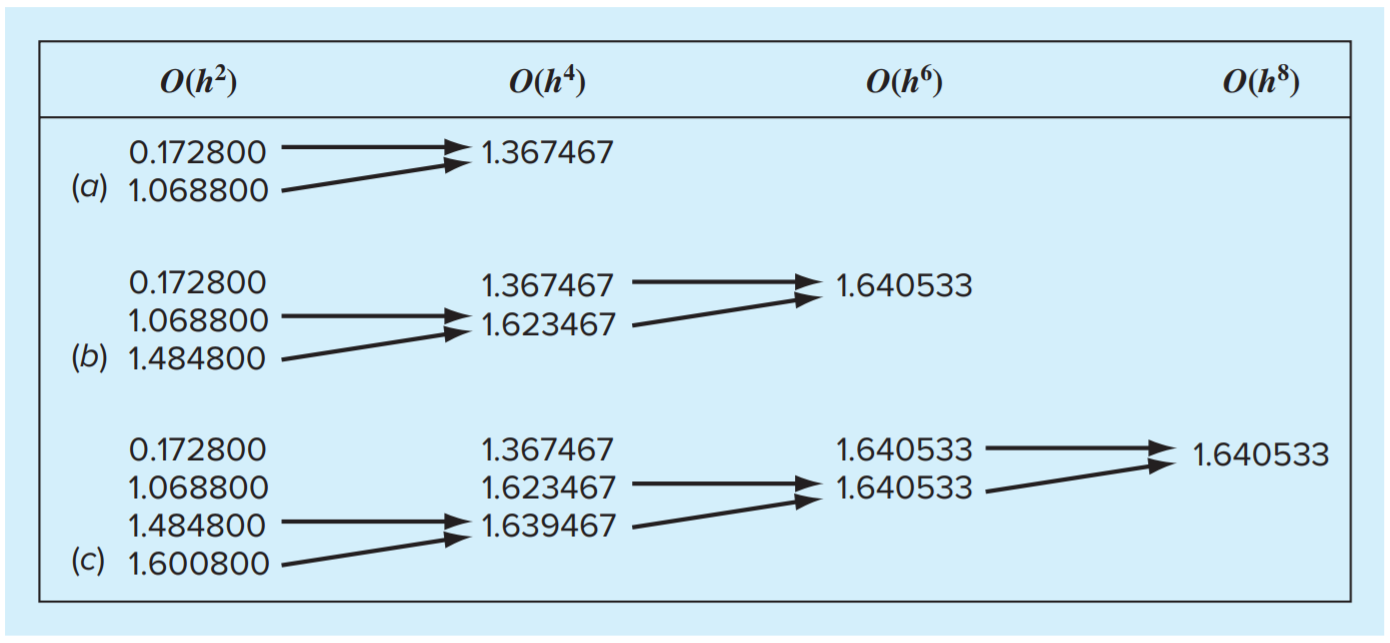
\includegraphics[width = 0.9\textwidth]{figures/RI}
	\end{figure}
\end{frame}

\begin{frame}
	\frametitle{$\mathcal{O}(h^4)$ Romberg Method Pseudocode}
	Download the \texttt{TrapezoidalRule.cpp} file from Canvas. We are going to modify it to contain the Romberg Method pseudocode.\\\vspace{10pt}
	
	\texttt{define function that takes in a, b, and tol}\\
	\texttt{declare/define error}\\
	\texttt{declare/define n = 1}\\
	\texttt{declare/define Il = TrapezoidalRule(a,b,n)}\\
	\texttt{declare/define Ik = 0, Im = 0}\\
	\texttt{declare/define k = 2}\\
	\texttt{ }\\
	\texttt{loop while error is greater than the tolerance}\\
	\texttt{\qquad update n for next trapezoid rule call, n*=2 }\\
	\texttt{\qquad Find Im by calling Trapezoidal rule for new n,}\\
	\texttt{\qquad Im = TrapezoidalRule(a,b,n)}\\
	\texttt{\qquad Compute Ik = (pow(4,k-1)*Im-Il)/(pow(4,k-1)-1)}\\
	\texttt{\qquad Compute the error = abs((Ik-Im)/Ik)}\\
	\texttt{\qquad Update Il = Im}\\
	
\end{frame}
	

\end{document}
